\chapter{\label{chap:model}Modelo e Implementação}

Conforme visto na Seção~\ref{simulator:flow}, um sistema de simulação possui uma
série de componentes conceituais, cada um com suas responsabilidades bem
definidas. Para projetar um simulador, diversas abordagens e paradigmas poderiam
ser aplicadas. Neste estudo optou-se pelo paradigma de \textit{Programação
Orientada a Objetos}. Esta escolha se deu pelos seguintes motivos:

\begin{description}
  \item[Capacidade de Abstração]\hfill \\
    Conceitos da \textit{Programação Orientada a Objetos}, como classes,
    interfaces, polimorfismo, herança e sobrecarga permitem a realização de uma
    modelagem conceitual em alto nível de abstração, permitindo uma explanação
    de fácil entendimento sem ser necessário abordar questões da implementação
    em si (linguagem de programação, arquitetura, etc).
  \item[Padrão de Mercado]\hfill \\
    Desde meados dos anos 90, a \textit{Programação Orientada a Objetos}
    tornou-se frequentemente utilizada no mercado de desenvolvimento de software
    e nos ambientes acadêmicos relacionados à computação. Assim, é possível
    atingir uma maior audiência.
  \item[Domínio dos Autores]\hfill \\
    O paradigma é de domínio dos autores deste estudo.
  \item[Suporte nativo no \texttt{C++}]\hfill \\
    O paradigma é suportado de forma no \texttt{C++11}, linguagem escolhida para
    a implementação.
\end{description}

Nas próximas seções serão apresentados os modelos\footnote{Algumas
simplificações foram realizadas nos modelos UML a fim de permitir uma melhor
compreensão~-~por exemplo, omissão de métodos \textit{getters} e
\textit{setters}.} e detalhes de implementação dos componentes genéricos de um
simulador. Após isto, serão apresentados os componentes específicos de um
simulador de elevadores.

\section{\label{model:events}Eventos}

A simulação de eventos discretos, como o próprio nome já diz, é orientada a
eventos. Isso significa dizer que as alterações no estado do sistema ocorrerão
somente na ocasião de algum evento e é preciso ser possível representar um
evento no contexto do simulador. Um evento é uma estrutura que deve possuir as
seguintes informações: (1) um número identificador; (2) o horário agendado para
a ocorrência do evento; (3) o tipo do evento.

Existem dois tipos de eventos que podem ocorrer durante uma simulação:

\begin{description}
  \item[Chegada de cliente] Um cliente chegou na fila de um andar.

  \item[Fim da simulação] A simulação atingiu a duração
especificada.\footnote{Este evento não necessariamente implica no fim imediato
da simulação, apenas que a chegada de novos clientes não ocorrerá mais. O
simulador ainda irá processar os clientes que estiverem nos andares ou dentro de
elevadores.}

\end{description}

Para obter tal funcionalidade foram criadas a classe abstrata \texttt{Event} e
as classes concretas que a especializam, representando os eventos de
\textbf{chegada de cliente} e \textbf{fim da simulação}, respectivamente:
\texttt{ClientArrival} e \texttt{FinishSimulation}
(Figura~\ref{fig:diagram:events}).

\begin{figure}[htb!]
  \centering
  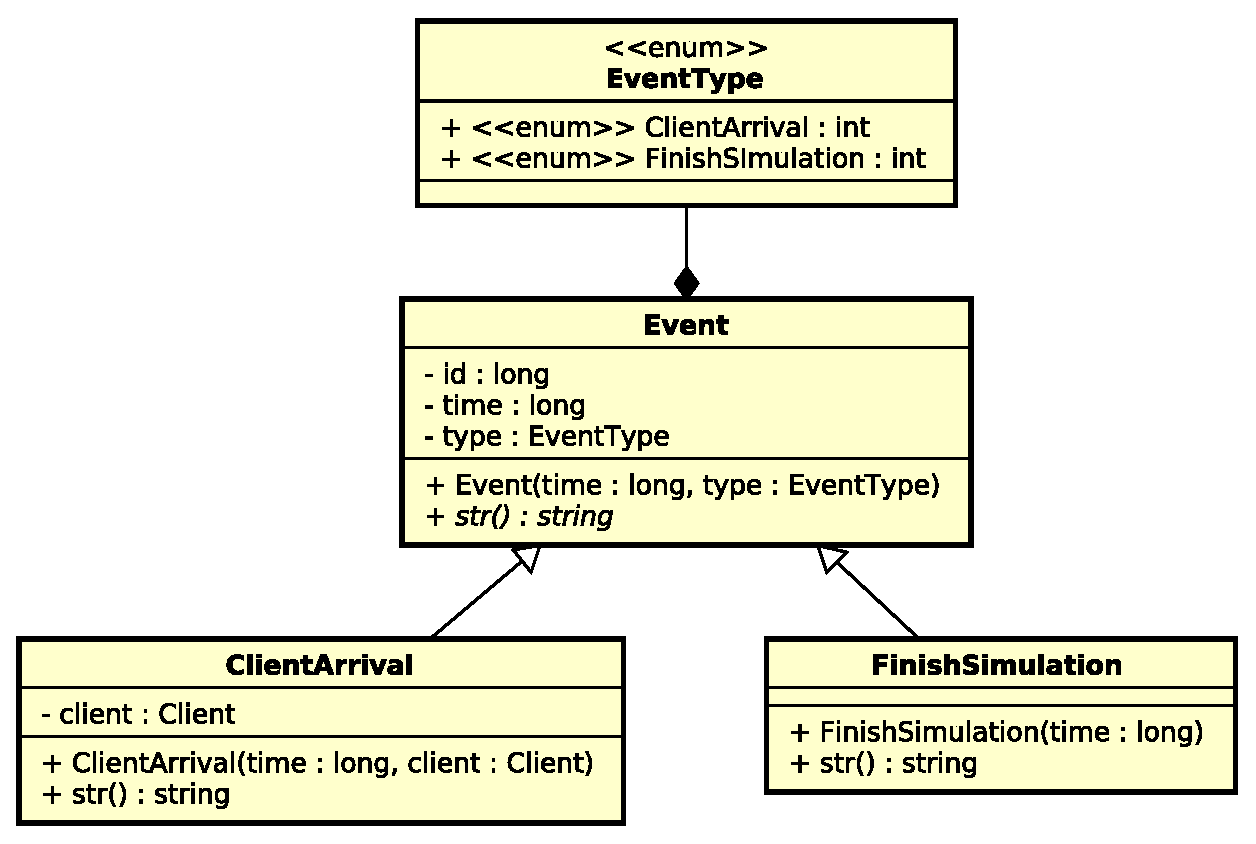
\includegraphics[scale=0.6]{img/Events}
  \caption{Diagrama de classes dos \textit{eventos e seus derivados}.}
\label{fig:diagram:events}
\end{figure}

\begin{description}
  \item[Event] \hfill \\
    Evento base composto pelo conjunto básico de informações para um evento.

    \begin{description}[leftmargin=!,labelwidth=\widthof{\bfseries client}]
      \item[\texttt{id}] Número identificador do evento.
      \item[\texttt{time}] Horário de ocorrência do evento.
      \item[\texttt{type}] Tipo do evento.
    \end{description}

  \item[ClientArrival] \hfill \\
    Evento especializado do tipo \textbf{chegada de cliente}. Contém,
    adicionalmente, as informações do cliente.

    \begin{description}[leftmargin=!,labelwidth=\widthof{\bfseries client}]
      \item[\texttt{client}] Cliente que gerou o evento.\footnote{Tipo complexo armazenando diversas informações sobre o cliente (Seção \ref{model:state:client}).}
    \end{description}

  \item[FinishSimulation] \hfill \\
    Evento especializado do tipo \textbf{fim da simulação}. Não é necessária
    nenhuma informação adicional.
\end{description}

\section{\label{sec:model:event}Gerenciamento de eventos}

Na Seção~\ref{simulator:flow} foram apresentados os componentes de um simulador.
Alguns destes componentes devem reagir na ocorrência de um evento, alterando o
seu estado interno de acordo com o tipo de evento ocorrido e as informações que
ele carrega consigo. Porém resta saber qual evento será o próximo a ocorrer e
como notificar os elementos reativos disso. Portanto, precisamos de mecanismos
para criar e ordenar eventos e notificar os componentes da ocorrência de um
evento.

\subsection{Criação} \label{model:event:creation}

Não é possível prever em qual andar e qual momento um cliente irá chegar ao
prédio, tampouco qual o destino desejado por ele. Portanto, é correto afirmar
que a chegada de clientes em um prédio é um processo estocástico.

\begin{description}

\item[Horário de chegada] \hfill \\
Segundo~\cite{Ross:2006:IPM:1197141}, a taxa de chegada de clientes é um
processo de Poisson, com razão $\lambda$. Ou seja, o tempo entre novos clientes
são variáveis independentes, com valor esperado $\frac{1}{\lambda}$. Pode-se ver
na Figura~\ref{fig:distribution:poisson} um exemplo de diferentes valores de
$\lambda$ gerando diferentes distribuições.

\begin{figure}[htb!]
  \centering
  \includegraphics[scale=1.0]{img/poisson.eps}
  \caption{Exemplos de distribuições de Poisson.}
\label{fig:distribution:poisson}
\end{figure}

Em um prédio no mundo real, esta distribuição varia de acordo com a hora do dia.
Por exemplo, nos horários do início do turno da manhã e no início do turno da
tarde, muito mais passageiros chegam ao térreo, com destino ao andar onde
trabalham. Para fim de simplificação, esta variação ao longo do dia não foi
considerada neste estudo. Conforme visto na Seção \ref{model:scenario}, cada
andar do prédio possui um valor para $\lambda$, que permanece constante no
decorrer de toda a simulação.

\item[Andar de destino] \hfill \\
Já a probabilidade de um cliente ir de um andar para outro, em um tráfego
chamado de \textit{interfloor}, é um processo de Markov, com distribuições
normais (\textit{i.e.} uma média e um desvio padrão) que variam de acordo com a
hora do dia. Para fim de simplificação, esta variação ao longo do dia não foi
considerada neste estudo. Além disso, considera-se que a probabilidade de um
cliente ir para qualquer andar é a mesma - com exceção do próprio em que se
encontra, que é nula. Abaixo uma matriz de probabilidades para um prédio com 3
andares, representada por uma cadeia de Markov na Figura
\ref{fig:distribution:markov}.

\[
  \begin{bmatrix}
    f_{11} & f_{12} & f_{13}  \\
    f_{21} & f_{22} & f_{23}  \\
    f_{31} & f_{32} & f_{33}
  \end{bmatrix} = \begin{bmatrix}
    0.0 & 0.5 & 0.5  \\
    0.5 & 0.0 & 0.5  \\
    0.5 & 0.5 & 0.0
  \end{bmatrix}
\]

\begin{figure}[htb!]
  \centering
  \includegraphics[scale=0.4]{img/markov.eps}
  \caption{Exemplo de cadeia de Markov para um prédio de 3 andares.}
\label{fig:distribution:markov}
\end{figure}

\item[EventFactory] \label{model:eventfactory} \hfill \\
A classe \texttt{EventFactory}, ou \textit{fábrica de eventos}, foi criada para
ser uma unidade de coesão ao criar chegadas de clientes no prédio. Cada andar do
prédio possui uma instância desta classe. Seus componentes são:

  \begin{description}[leftmargin=!,labelwidth=\widthof{\bfseries hasNextEvent}]
    \item[\texttt{clock}] Referência para o relógio da simulação.
    \item[\texttt{floor}] Referência para o andar daquele \texttt{EventFactory}.
    \item[\texttt{random engine}] Gerador de números aleatórios.
    \item[\texttt{destination}] Distribuição Discreta, utilizada para sortear andares de destino.
    \item[\texttt{arrival}] Distribuição de Poisson, utilizada para sortear horários de eventos futuros.
  \end{description}

  O Algoritmo \ref{alg:eventcreation} ilustra a criação de um novo evento.
  Primeiro, \texttt{CreateFutureArrival} calcula o horário do novo evento. Isto
  é feito somando-se o horário atual do \textit{relógio da simulação} com um
  tempo sorteado pela distribuição de Poisson específica daquele andar. Na
  sequência, é sorteado o andar de destino pela distribuição discreta também
  específica do andar. Feito isso, é criado um novo evento do tipo
  \textbf{chegada de cliente} com as informações sorteadas e tendo como origem o
  andar atual. No fim, o evento criado é adicionado à fila de eventos (Seção
  \ref{model:queue}).
    \begin{algorithm}[htb!]
      \centering
        \begin{minted}[linenos,fontsize=\small]{c++}
EventFactory::createFutureArrival(EventQueue eventQueue) {
  eventTime = clock.currentTime() + getNextTime();
  destination = getNextDestination();
  clientArrival = new ClientArrival(floor, destination, eventTime);
  eventQueue.push(clientArrival);
}

EventFactory::getNextTime() {
  return arrival(randomEngine);
}

EventFactory::getNextDestination() {
  return destination(randomEngine);
}
        \end{minted}
      \caption{\label{alg:eventcreation}Criação de um novo \textit{evento de chegada de cliente}.}
    \end{algorithm}
\end{description}

\subsection{Priorização} \label{model:queue}

Na Seção~\ref{simulator:movation:discrete} foi apresentado o \textit{mecanismo
de avanço de tempo para o próximo evento}, onde deve-se verificar, em uma lista
de eventos, qual é o próximo evento a ocorrer. Dado um conjunto de eventos
agendados (ou seja, ainda não ocorridos), o primeiro evento a ocorrer é
justamente o que possui o menor tempo de agendamento. Um tipo abstrato de dados
que serve para este propósito é uma \textit{fila prioritária}, ou
\textit{priority queue}, que funciona de forma similar a filas \textit{FIFO},
com a diferença de que cada elemento armazenado possui uma prioridade associada.
A \textit{fila prioritária}, implementada na classe \texttt{EventQueue}, irá
atender os elementos por ordem de prioridade, da maior para a menor. Ao
considerar que a prioridade de um evento é inversamente proporcional ao instante
em que irá ocorrer - ou seja, quanto menor o tempo do evento maior é a sua
prioridade -, temos uma fila na qual o próximo elemento a ser atendido sempre
será o próximo evento a ocorrer.

\begin{description}
  \item[EventQueue] \hfill \\
    Encapsula uma fila prioritária de eventos. Adicionalmente, utiliza a classe
    \texttt{EventComparator}, que implementa a relação de ordem entre os
    eventos.

    \begin{description}[leftmargin=!,labelwidth=\widthof{\bfseries hasNextEvent}]
      \item[\texttt{push}] Insere um evento na fila.
      \item[\texttt{top}] Recupera o próximo evento da fila.
      \item[\texttt{pop}] Recupera e remove o próximo evento da fila.
      \item[\texttt{hasNextEvent}] Verifica se a fila possui eventos.
    \end{description}
\end{description}

\begin{figure}[htb!]
  \centering
  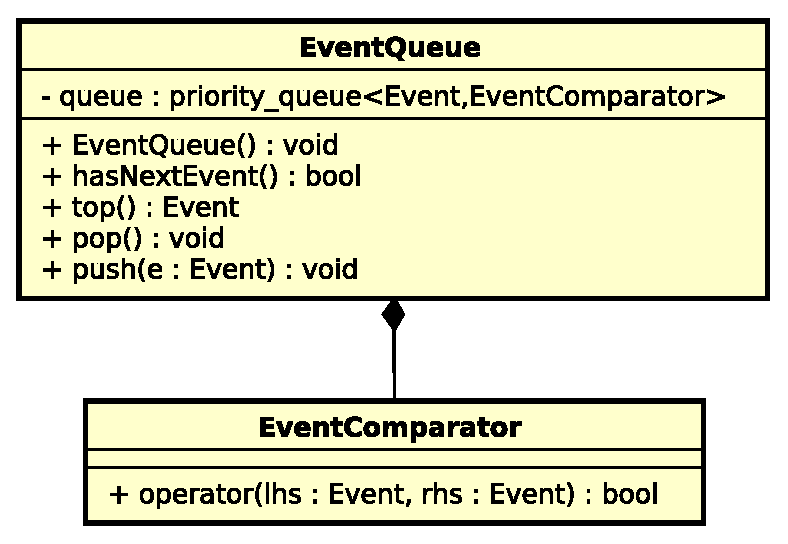
\includegraphics[scale=0.6]{img/EventQueue}
  \caption{Diagrama de classes da \textit{criação e priorização de eventos}.}
\label{fig:diagram:event:manage}
\end{figure}

\subsection{Notificação}

Quando o próximo evento a ocorrer é conhecido, o problema passa a ser notificar
os elementos reativos que este evento ocorreu para que os mesmos possam
atualizar seus estados internos. De acordo com Gamma
\cite{Gamma:1995:DPE:186897}, o padrão \textit{Observer} é um \textit{design
pattern} indicado para resolver este problema. Este \textit{pattern} define uma
dependência de um-para-muitos ($1:N$) entre objetos de modo que, quando este um
objeto (\textit{subject}) tem seu estado alterado, todos os seus dependentes
(\textit{observers}) são notificados deste mudança. Por consequência, estes
dependentes podem modificar seu estado interno baseando-se nas informações desta
notificação.

Este padrão foi utilizado para implementar a funcionalidade de notificação de
eventos, ilustrado no diagrama da Figura~\ref{fig:diagram:notification}. Para
isto, foram criados os seguintes componentes:

\begin{figure}[htb!]
  \centering
  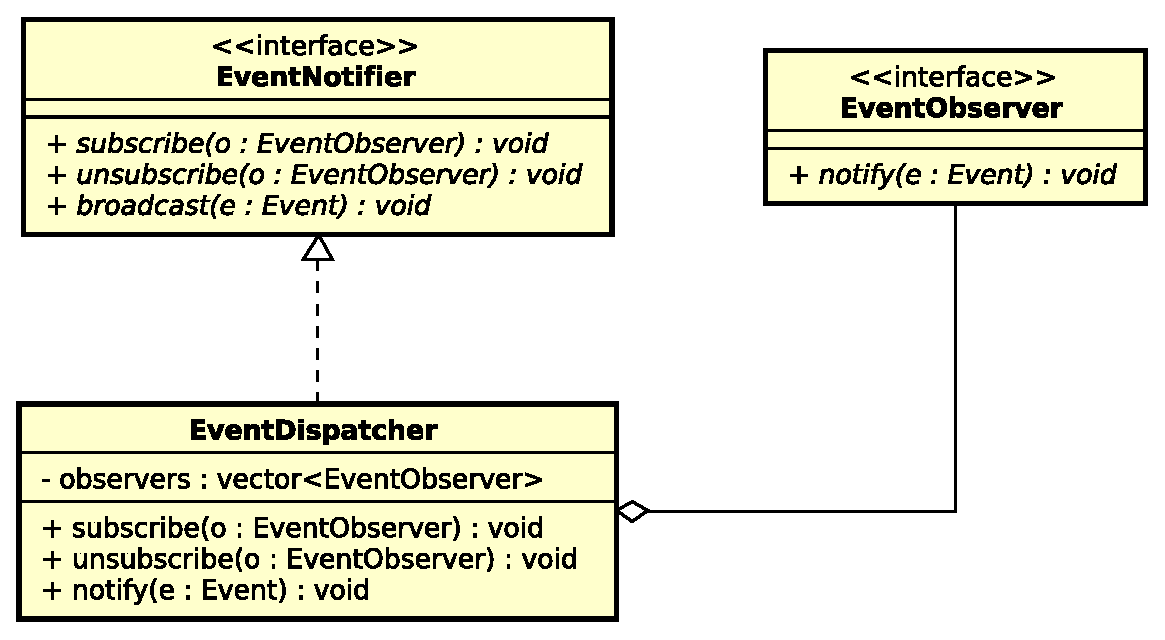
\includegraphics[scale=0.6]{img/EventNotifier}
  \caption{Diagrama de classes da \textit{notificação de eventos}.}
\label{fig:diagram:notification}
\end{figure}

\begin{description}
  \item[EventObserver] \hfill \\
    Classe abstrata a ser realizada por qualquer outra classe que deseje receber
    notificações de eventos. Possui um único método abstrato.

    \begin{description}[leftmargin=!,labelwidth=\widthof{\bfseries unsubscribe}]
      \item[\texttt{notify}] Recebe a notificação da ocorrência de um evento.
    \end{description}

  \item[EventNotifier] \hfill \\
    Classe abstrata a ser realizada por qualquer outra classe que deseje
    notificar a ocorrência de eventos. Define métodos para que objetos que
    implementem a classe abstrata \textit{EventObserver} possam registrar-se
    para receber notificações de ocorrências de eventos. Seus métodos abstratos
    são:

    \begin{description}[leftmargin=!,labelwidth=\widthof{\bfseries unsubscribe}]
      \item[\texttt{subscribe}] Adiciona um \textit{observer}.
      \item[\texttt{unsubscribe}] Remove um \textit{observer}.
      \item[\texttt{broadcast}] Notifica todos os \textit{observers} registrados da ocorrência de um evento.
    \end{description}

  \item[EventDispatcher] \hfill \\
    Classe concreta que realiza a interface \texttt{EventNotifier}. Possui uma
    estrutura de dados para armazenar quais \textit{observers} se registraram
    através dos métodos \texttt{subscribe} e \texttt{unsubscribe}.
\end{description}

Três importantes componentes do simulador podem se beneficiar desta construção:
(1) o \textit{relógio do sistema} (classe \texttt{Clock}); (2) os
\textit{contadores estatísticos} (classe \texttt{Statistics}); e (3) o
\textit{estado do sistema} (classe \texttt{Building}). Na ocorrência de um
evento, estas três entidades devem ser notificadas e cada uma irá alterar seu
estado interno da forma adequada. Para isto, devem implementar a interface
\texttt{EventObserver} e registrarem-se no \texttt{EventDispatcher}. Assim, o
\texttt{EventDispatcher} e a \texttt{EventQueue} podem, juntos, notificar aos
componentes reativos exatamente qual evento ocorreu em cada iteração da
simulação, na ordem correta dos eventos.

\section{Relógio da simulação} Durante a execução da simulação, à medida que
eventos ocorrem, componentes do simulador devem alterar seu estado interno de
acordo com o evento ocorrido, levando o estado do simulador a uma nova situação.
Um destes componentes é o \textit{relógio da simulação}. Portanto, deve realizar
a classe concreta \texttt{EventObserver}.

O \textit{relógio da simulação} é representado pela classe \texttt{Clock}
(Figura~\ref{fig:diagram:clock}). Esta classe encapsula o atributo privado
\texttt{time} e provê métodos para sua consulta e atualização.

\begin{figure}[htb!]
  \centering
  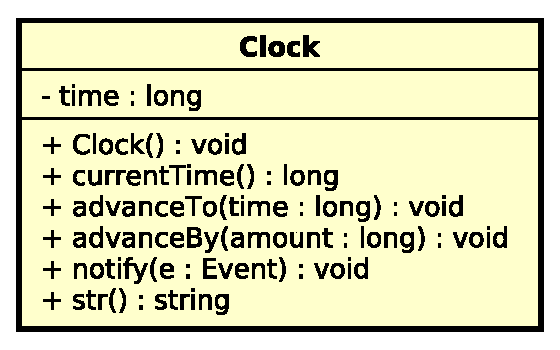
\includegraphics[scale=0.6]{img/Clock}
  \caption{Diagrama de classes do \textit{relógio do sistema}.}
\label{fig:diagram:clock}
\end{figure}

\begin{description}[leftmargin=!,labelwidth=\widthof{\bfseries currentTime}]
  \item[\texttt{currentTime}] Retorna o horário atual do \textit{relógio da simulação}.
  \item[\texttt{advanceTo}] Avança o \textit{relógio da simulação} para um horário arbitrário.
  \item[\texttt{advanceBy}] Avança o \textit{relógio da simulação} em uma quantidade arbitrária de segundos.
  \item[\texttt{str}] Representação textual do \textit{relógio da simulação} (utilizado em \textit{logs}).
  \item[\texttt{notify}]
  Realização da classe abstrata \texttt{EventObserver}. Ao ser notificado de um
  evento, o \textit{relógio da simulação} deve avançar o relógio interno para o
  instante da ocorrência do evento, independentemente do tipo de evento que
  ocorreu. O Algoritmo \ref{alg:advanceto} ilustra este conceito.
\end{description}

\begin{algorithm}[htb!]
  \centering
    \begin{minted}[linenos,fontsize=\small]{c++}
Clock::notify(Event event) {
  eventTime = event.getTime();
  advanceTo(eventTime);
}
    \end{minted}
  \caption{\label{alg:advanceto}\textit{Relógio do sistema} reagindo a um evento.}
\end{algorithm}

\section{Contadores estatísticos}

Os \textit{contadores estatísticos} da simulação são responsáveis por coletar e
sumarizar dados do sistema durante toda a execução da simulação. Sua existência
permite a realização de análises qualitativas e quantitativas a respeito do
sistema simulado. Assim como o \textit{relógio da simulação}, os
\textit{contadores estatísticos} também devem ter o seu estado alterado na
ocorrência de eventos. Portanto, devem realizar a classe concreta
\texttt{EventObserver}.

Neste projeto, os \textit{contadores estatísticos} são
representados pelas estruturas \texttt{Arrival} e \texttt{Trip} e pela classe
\texttt{Statistics} (Figura~\ref{fig:diagram:statistics}).

\begin{figure}[htb!]
  \centering
  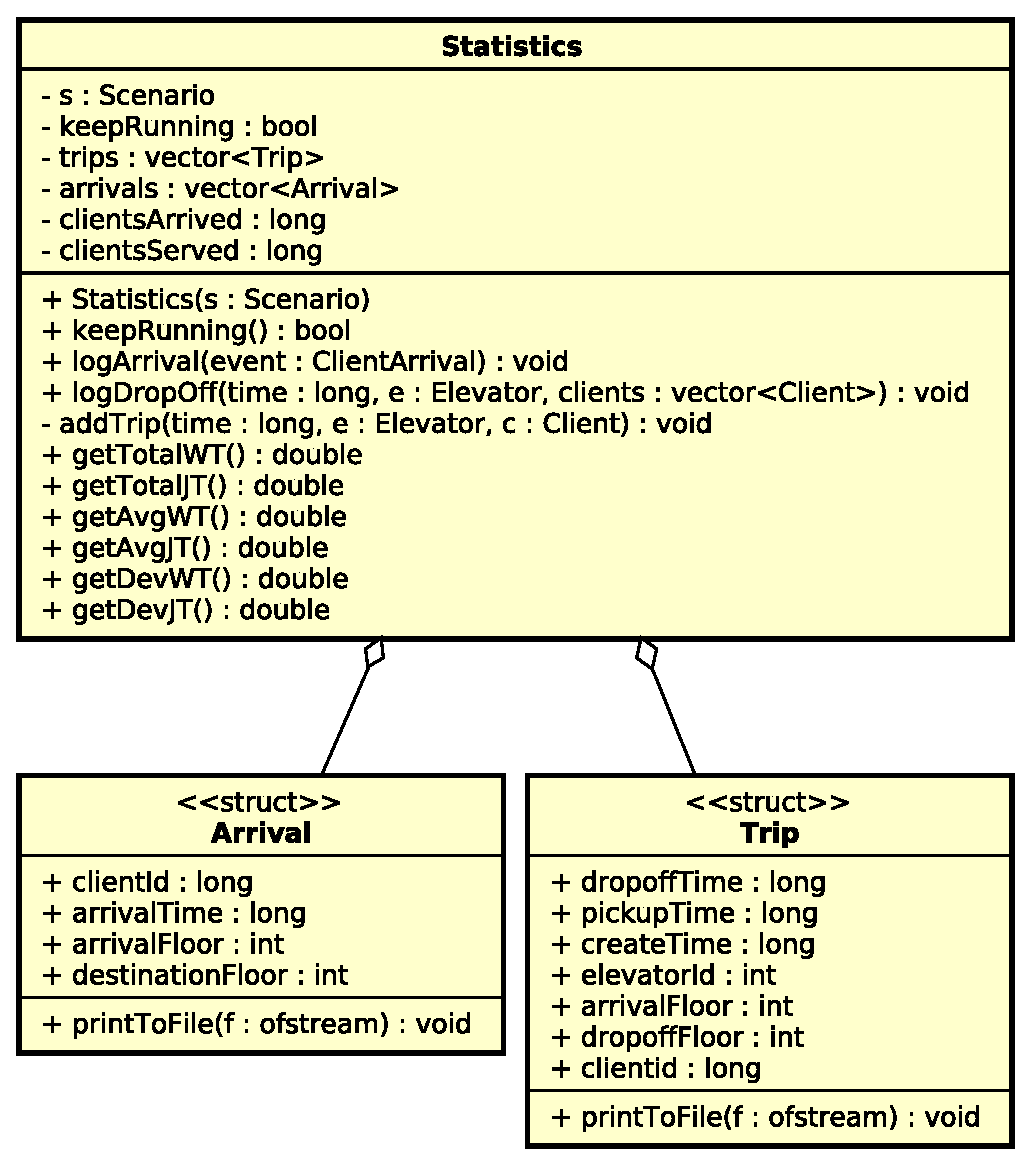
\includegraphics[scale=0.6]{img/Statistics}
  \caption{Diagrama de classes dos \textit{contadores estatísticos}.}
\label{fig:diagram:statistics}
\end{figure}

\begin{description}
  \item[Arrival] \hfill \\
    Uma instância desta estrutura armazena informações coletadas quando um
    cliente chega ao prédio. Tais informações são:

    \begin{description}[leftmargin=!,labelwidth=\widthof{\bfseries destinationFloor}]
      \item[\texttt{clientId}] Número identificador do cliente.
      \item[\texttt{arrivalTime}] Horário em que o cliente chegou ao prédio.
      \item[\texttt{arrivalFloor}] Número do andar no qual o cliente chegou.
      \item[\texttt{destinationFloor}] Andar de destino ao qual o cliente deseja dirigir-se.
    \end{description}

  \item[Trip] \hfill \\
    Uma instância desta estrutura armazena informações coletadas quando um
    cliente desembarca de um elevador. Tais informações são:

    \begin{description}[leftmargin=!,labelwidth=\widthof{\bfseries destinationFloor}]
      \item[\texttt{clientId}] Número identificador do cliente.
      \item[\texttt{dropoffTime}] Horário em que o cliente desembarcou do elevador.
      \item[\texttt{createTime}] Horário em que o cliente chegou ao prédio.
      \item[\texttt{elevatorId}] Número do elevador do qual o cliente desembarcou.
      \item[\texttt{arrivalFloor}] Número do andar no qual o cliente chegou.
      \item[\texttt{dropoffFloor}] Número do andar no qual o cliente desembarcou.
    \end{description}

  \item[Statistics] \hfill \\
    Armazena as estatísticas coletadas durante a simulação e fornece
    estatísticas sobre os dados coletados no fim da simulação. Seus
    métodos são:

    \begin{description}[leftmargin=!,labelwidth=\widthof{\bfseries destinationFloor}]
      \item[\texttt{logDropOff}] Registra a ocorrência de um desembarque.
      \item[\texttt{logTrip}] Registra a ocorrência de uma chegada de um cliente.
      \item[\texttt{getAvgWT}] Calcula o tempo de espera médio.
      \item[\texttt{getDevWt}] Calculo o desvio padrão do tempo de espera.
      \item[\texttt{getTotalWT}] Calcula o tempo de espera total.
      \item[\texttt{getAvgWT}] Calcula o tempo de jornada médio.
      \item[\texttt{getDevWt}] Calcula o desvio padrão do tempo de jornada.
      \item[\texttt{getTotalWT}] Calcula o tempo de jornada total.
      \item[\texttt{keepRunning}] Avalia se a simulação deve terminar\footnote{por exemplo, se o tempo de duração da simulação já se passou.}.
      \item[\texttt{notify}]
        Realização da classe abstrata \texttt{EventObserver}. Ao ser notificado
        de um evento: se for do tipo \textbf{chegada de cliente}, deve coletar e
        armazenar as informações desta nova chegada; se for do tipo \textbf{fim
        da simulação}, deve altera o estado do atributo privado
        \texttt{keepRunning} para \texttt{false}. Esta ação irá interromper a
        chegada de novos clientes. O Algoritmo \ref{alg:statistics} ilustra este
        conceito.
    \end{description}

\begin{algorithm}[htb!]
  \centering
    \begin{minted}[linenos,fontsize=\small]{c++}
Statistics::notify(Event event) {
  if (event.getType() == ClientArrival) {
    logArrival(event);
  }

  if (event.getType() == FinishSimulation) {
    keepRunning = false;
  }
}
    \end{minted}
  \caption{\label{alg:statistics}\textit{Contadores estatísticos} reagindo a um evento.}
\end{algorithm}

\end{description}

\section{\label{model:simulador}Simulador}

O uso conjunto de todos estes componentes e classes dá forma ao simulador,
conforme proposto por \cite{Law,Banks}. Entretanto, todas as interações entre as
instâncias devem ser organizadas conforme o fluxo proposto na Figura
\ref{fig:simflow}. O componente responsável por orquestrar estas interações e
garantir o fluxo de execução é representado pela classe \textit{Simulator}. Esta
classe não possui atributos ou métodos específicos; somente as instâncias das
outras classes e um método que implementa o laço de execução do simulador.

\begin{figure}[htb!]
  \centering
  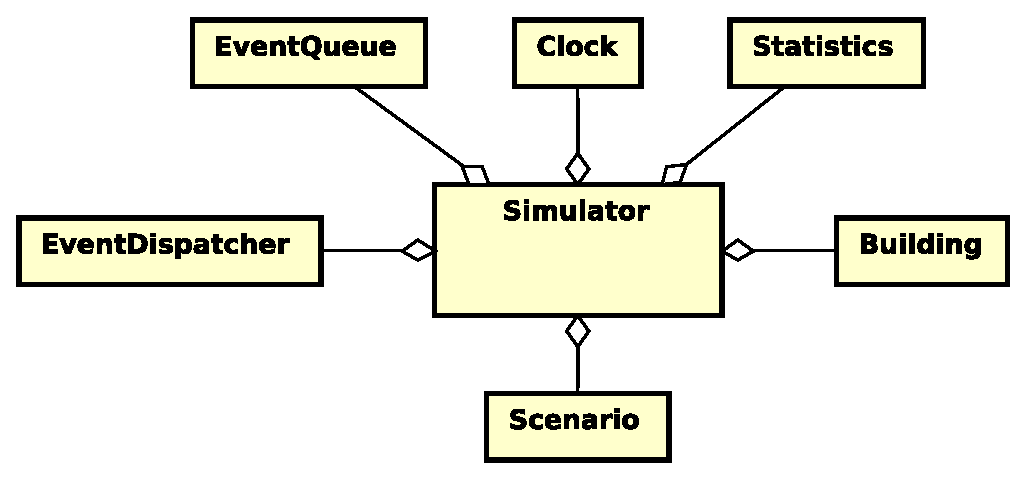
\includegraphics[scale=0.6]{img/Simulator}
  \caption{Diagrama de classes do simulador.}
\label{fig:diagram:simulator}
\end{figure}

O Algoritmo \ref{alg:sim} mostra como funciona o laço de execução da simulação.
Na linha 2, uma instância da classe \texttt{Building} (Seção
\ref{model:state:building}) é criada baseada nos atributos definidos para o
cenário \ref{model:scenario}. Nas linhas 4 a 6, os objetos \textit{observers} se
registram no \textit{notifier} para receberem notificações de eventos. É
importante frisar que a ordem na qual se registram é a mesma ordem na qual serão
notificados da ocorrência de eventos. Nas linhas 8 a 10, é criado um evento para
marcar o fim da simulação e o mesmo é adicionado à \textit{fila de eventos}. Na
linha 12, são inicializados os eventos de chegada de clientes em cada um dos
andares (Seção \ref{model:state:building}). Por fim, o simulador entra em um
laço indefinido nas linhas 14 a 17. A cada iteração do laço é retirado o próximo
evento da fila e os \textit{observers} são notificados. O laço permanece em
execução enquanto houver eventos disponíveis na fila ou até atingir o tempo
limite da simulação.

\begin{algorithm}[htb!]
  \centering
    \begin{minted}[linenos,fontsize=\small]{c++}
Simulator::run() {
  building = new Building(scenario);

  dispatcher.subscribe(building);
  dispatcher.subscribe(clock);
  dispatcher.subscribe(statistics);

  duration = scenario.getDuration();
  finishSimulation = new FinishSimulation(duration);
  eventQueue.push(finishSimulation);

  building.initializeClientArrivals(eventQueue);

  while (statistics.keepRunning() and eventQueue.hasNextEvent()) {
    nextEvent = eventQueue.pop();
    dispatcher.broadcast(nextEvent);
  }
}
    \end{minted}
  \caption{\label{alg:sim}Laço de execução da simulação.}
\end{algorithm}

\section{\label{model:scenario}Cenário}

Até este ponto foram apresentados componentes genéricos de um simulador. A
partir daqui serão detalhados componentes específicos de um simulador de
elevadores. O primeiro deles é o \textit{cenário}. Como entrada o simulador
recebe um conjunto de cenários e realiza a simulação de cada um deles. Um
cenário é composto pelas seguintes informações:

\begin{description}[leftmargin=!,labelwidth=\widthof{\bfseries Função de Custo}]
  \item[Nome]
  Identificação textual do cenário.

  \item[Duração]
  Quantidade de unidades de tempo durante a qual serão geradas chegadas de
  clientes aos andares do prédio. Após esta duração, não chegarão mais clientes.
  Porém, clientes que já entraram no prédio e estão distribuídos nos andares e
  elevadores precisam terminar suas viagens antes que a simulação chegue ao fim.
  Devido a isto, é normal que o duração final seja maior que a duração
  estipulada no cenário.

  \item[Agendamento]
  Lista de algoritmos de agendamento.

  \item[Horizonte]
  Horizonte de expansão do agendamento com algoritmo de \textit{planning}.

  \item[Função de Custo]
  Lista de funções de custo.

  \item[Semente]
  Semente textual para inicialização os geradores de números aleatórias.

  \item[Elevadores]
  Número de elevadores do prédio.

  \item[Capacidade]
  Capacidade dos elevadores (a mesma para cada elevador).

  \item[Andares]
  Lista com o intervalo médio\footnote{O valor médio informado é utilizado como
  parâmetro $\lambda$ de entrada para uma Distribuição de Poisson. Cada andar do
  prédio possui uma distribuição distinta.} de chegada de passageiros, em
  segundos, para cada andar. A lista começa com a média do andar térreo e segue
  sucessivamente. O número de andares é igual ao tamanho da lista.

\end{description}

O parâmetro \textit{função de custo} será utilizado no agendamento
\textit{Simple}\footnote{Será realizada uma simulação para cada função de
custo.} e o parâmetro \textit{horizonte} no agendamento \textit{Planning}.

\subsection{\label{model:scenario:config}Arquivo de Configuração}

A entrada de dados para o simulador se dá através de um arquivo de configuração
chamado \texttt{config.yaml}. Este arquivo obedece o padrão \textit{YAML}, um
formato de serialização de dados legíveis por humanos.

\begin{listing}[htb!]
  \centering
    \begin{minted}[linenos,fontsize=\small]{yaml}
scenarios:
  - name: Scenario 1
    duration: 86400
    scheduler: [ 0, 1 ] # simple, planning
    planningHorizon: 5
    cost_function: [ 0, 2, 3 ] # randon, bnn, weighted
    seed: 54TH7hboAG1iOsDIDhJp
    elevators: 2
    capacity: 6
    floors: [ 60, 520, 360, 240, 240, 90, 90, 90 ]

  - name: Scenario 2
    # ...

  - name: Scenario N
    # ...
    \end{minted}
  \caption{Exemplo de arquivo de configuração \texttt{config.yaml}.}
  \label{alg:config}
\end{listing}

No exemplo da Listagem~\ref{alg:config} são definidos alguns cenários. No
primeiro, chamado \texttt{Scenario 1}, clientes chegarão durante 12 horas
distribuídos ao longo dos 8 andares do prédio e serão atendidos por 2
elevadores, cuja capacidade é de 8 passageiros cada. Pode ser definido um número
ilimitado de cenários no arquivo de entrada.

Para representar as informações referentes a um cenário foi criada a classe
\texttt{Scenario} (Figura~\ref{fig:diagram:scenario}). Além de armazenar as
informações, disponibiliza o método \texttt{Load}, cujo objetivo é carregar os
cenários a partir do arquivo de configuração utilizando a biblioteca \texttt
{yaml-cpp}.

\begin{figure}[htb!]
  \centering
  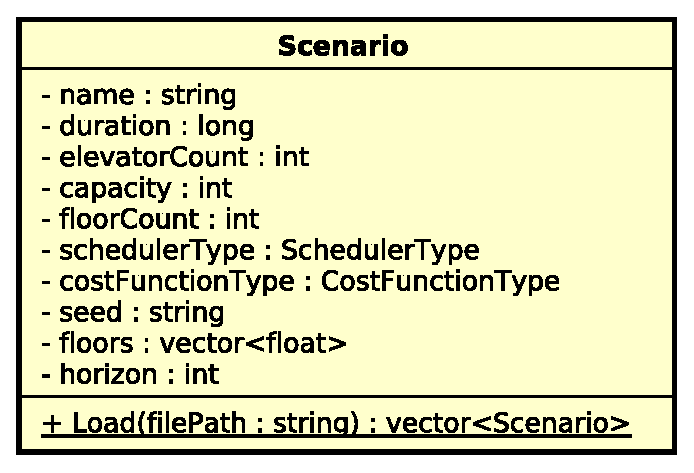
\includegraphics[scale=0.6]{img/Scenario}
  \caption{Diagrama de classes dos \textit{cenários}.}
\label{fig:diagram:scenario}
\end{figure}

\section{Estado do sistema}

Entre os componentes fundamentais de um simulador destaca-se a representação do
\textit{estado do sistema}, uma coleção de objetos e variáveis necessárias para
descrever o sistema em um instante em particular da simulação~\cite{Law}. Neste
projeto, a classe \texttt{Building} é responsável por encapsular o conjunto de
informações que definem este estado (Figura~\ref{fig:diagram:model}). Esta
classe é responsável por gerenciar múltiplas instâncias de elevadores (classe
\texttt{Elevator}), andares (classe \texttt{Floor}) e clientes (classe
\texttt{Client}) e relacionar estas instâncias entre si - reproduzindo, deste
modo, as dinâmicas do sistema do mundo real que está sendo simulado.

\subsection{Cliente} \label{model:state:client}
  Uma pessoa que chegou a um andar e deseja se dirigir a outro andar é
  representada, dentro do simulador, por um objeto da classe \texttt{Client}.
  Possui os seguintes atributos:

  \begin{description}[leftmargin=!,labelwidth=\widthof{\bfseries arrivalFloor}]
    \item[\texttt{id}] Número identificador do cliente.
    \item[\texttt{destination}] Número do andar ao qual o cliente deseja dirigir-se.
    \item[\texttt{arrivalFloor}] Número do andar no qual o cliente chegou.
    \item[\texttt{createTime}] Horário em que o cliente chegou ao prédio.
    \item[\texttt{pickupTime}] Horário em que o cliente embarcou em um elevador.
  \end{description}

\subsection{Andar} \label{model:floor}

Parte componente de um prédio, representada pela classe \texttt{Floor}. Possui
os seguintes atributos:

  \begin{description}[leftmargin=!,labelwidth=\widthof{\bfseries eventFactory}]
    \item[\texttt{number}] Número do andar em que a parada deve ser realizada.
    \item[\texttt{lambda}] Valor de entrada para a distribuição de Poisson do andar.
    \item[\texttt{upLine}] Fila contendo os clientes que desejam subir\footnote{No mundo real, apesar de aparentemente as pessoas formarem
    uma fila única, os membros da fila respeitam o sentido de viagem do elevador
    e implicitamente separam-se em duas filas: uma para subir e outra para
    descer.} a partir do andar.
    \item[\texttt{downLine}] Fila contendo os clientes que desejam descer a partir do andar.
    \item[\texttt{eventFactory}] Instância da classe \texttt{EventFactory} (Seção \ref{model:eventfactory}) do andar.
  \end{description}

\subsection{Elevador}

  Um elevador é representado pela classe \texttt{Elevator}. Possui os seguintes
  atributos:

  \begin{description}[leftmargin=!,labelwidth=\widthof{\bfseries arrivalFloor}]
    \item[\texttt{number}] Número identificador do elevador.
    \item[\texttt{capacity}] Capacidade máxima do elevador (em número de clientes).
    \item[\texttt{location}] Número do andar no qual o elevador se encontra.
    \item[\texttt{destination}] Parada\footnote{Por exemplo, parar no andar 5 subindo é diferente de parar no andar 5 descendo.} de destino do elevador, composto pelo número do andar e a direção da parada.
    \item[\texttt{status}] Situação atual do elevador: \textit{moving} (movendo-se) ou \textit{idle} (ocioso).
    \item[\texttt{direction}] Direção na qual o elevador está se movendo (no caso de não estar ocioso).
    \item[\texttt{passengers}] Conjunto com os passageiros que embarcaram no elevador e ainda não desembarcaram.
  \end{description}

\subsection{Gerenciador de Paradas}

  Para tornar a tarefa de controlar paradas mais simples, foi criada uma classe
  auxiliar que implementa um gerenciador de paradas chamada
  \texttt{StopManager}. Expõe as seguintes funcionalidades:

  \begin{description}[leftmargin=!,labelwidth=\widthof{\bfseries arrivalFloor}]
    \item[\texttt{hasStop}] Verifica se há algum elevador programado para parar em dado andar e direção.
    \item[\texttt{set}] Adiciona uma parada em dado andar e direção à lista de paradas do elevador.
    \item[\texttt{clear}] Remove um parada em dado andar e direção da lista de paradas do elevador.
    \item[\texttt{getStops}] Retorna o conjunto de andares com paradas programadas para um elevador em dada direção.
  \end{description}

  \begin{figure}[htb!]
    \centering
    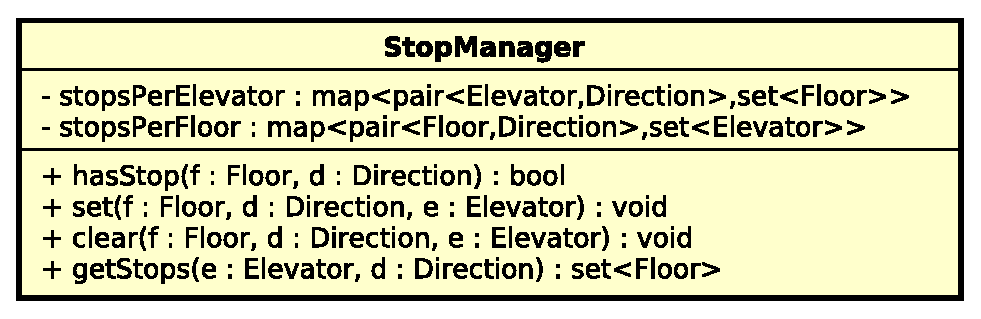
\includegraphics[scale=0.6]{img/StopManager}
    \caption{Diagrama de classes do \textit{gerenciador de paradas}.}
  \label{fig:diagram:stopmanager}
  \end{figure}

\subsection{Prédio} \label{model:state:building}

O \textit{prédio} sendo simulado é representado pela classe \texttt{Building}.
Esta classe agrupa os demais componentes do prédio, possuindo um conjunto de
andares e elevadores. Assim como o \textit{relógio da simulação} e os
\textit{contadores estatísticos}, o \textit{prédio} também terá seu estado
alterado na ocorrência de eventos. Portanto, a classe \texttt{Building} deve
implementar a interface para \textit{observers}. As responsabilidades desta
classe estão expostas para o simulador da seguinte forma:

\begin{description}
  \item[Inicializar a lista de chegadas de clientes] \hfill \\
    Conforme visto nas Seções \ref{model:event:creation} e \ref{model:floor}, há
    um objeto da classe \texttt{EventFactory} para cada objeto \texttt{Floor} do
    prédio. O objeto \texttt{Building} é responsável por realizar a invocação do
    \texttt{EventFactory} para criar novos eventos de chegada de cliente e
    adicioná-los à fila de eventos. O Algoritmo \ref{alg:building:init} mostra
    um excerto do código da classe \texttt{Building}, responsável por realizar
    esta inicialização. O método \texttt{initializeArrivals} itera por todos os
    andares do prédio e invoca a criação de um novo evento, passando como
    parâmetro um ponteiro para a fila de eventos para que o
    \texttt{EventFactory} consiga adicionar o evento recém criado (Algoritmo
    \ref{alg:eventcreation}).

    \begin{algorithm}[htb!]
      \centering
        \begin{minted}[linenos,fontsize=\small]{c++}
Building::initializeArrivals() {
  eventQueue = simulator.getEventQueue();
  for each (floor in floors)
    floor.createFutureArrival(eventQueue);
}
        \end{minted}
      \caption{Inicialização dos eventos de chegada de cliente.}
      \label{alg:building:init}
    \end{algorithm}

  \item[Reagir à ocorrência de eventos] \hfill \\
    Como o estado interno deve ser alterado na ocorrência de eventos, o
    \texttt{Building} implementa a interface \texttt{EventObserver} conforme o
    Algoritmo \ref{alg:building:notify}. Nas linhas 2 a 4 do método é feita a
    atualização do estado interno do prédio para refletir o que ocorreu no
    interim entre o momento do último evento processadoe o que está sendo
    notificado~-~como o \textit{prédio} recebe notificações antes do
    \textit{relógio do sistema}, o segundo ainda está no estado referente ao
    evento ocorrido anteriormente. Com o estado do prédio atualizado, o evento
    recebido pode ser processado de acordo com o seu tipo (linhas 7 e 11).

    \begin{algorithm}[htb!]
      \centering
        \begin{minted}[linenos,fontsize=\small]{c++}
Building::notify(Event event) {
  for (time = _clock.currentTime(); time < event.getTime(); ++time) {
    step();
  }

  if (event.getType() == ClientArrival) {
    doClientArrival(event);
  }

  if (event.getType() == FinishSimulation) {
    doFinishSimulation(event);
  }
}
        \end{minted}
      \caption{\textit{Prédio} reagindo a um evento.}
      \label{alg:building:notify}
    \end{algorithm}

  \item[Reagir à chegada de um novo cliente] \hfill \\
    O Algoritmo \ref{alg:building:arrival} ilustra como o \texttt{Building}
    trata o evento de \textit{chegada de cliente}. Nas linhas 2 a 4 são
    identificados o cliente, a direção em que irá se locomover e o andar em que
    ocorreu o evento de sua chegada. Na linha 5 o cliente é adicionado à fila do
    andar correspondente. Caso não exista uma parada programada de um elevador
    no andar e na direção (linha 7), será necessário escolher um elevador para
    atender este cliente. Neste momento, o \textit{algoritmo de agendamento} é
    invocado (linha 8) e a decisão é informada ao \textit{gerenciador de
    paradas} (linha 9). Por fim, nas linhas 12 a 13 é gerado um novo evento
    futuro de \textit{chegada de cliente} para o andar onde o evento ocorreu, de
    modo a repopular as filas de cada andar.

    \begin{algorithm}[htb!]
      \centering
        \begin{minted}[linenos,fontsize=\small]{c++}
Building::doClientArrival(ClientArrival event) {
  client = event.getClient();
  direction = client.getDirection();
  location = client.getArrivalFloor();
  location.addClient(client);

  if (!stopManager.hasStop(location, direction)) {
    elevator = scheduler.schedule(costFunction, building, client);
    stopManager.set(location, direction, elevator);
  }

  eventQueue = simulator.getEventQueue();
  location.createFutureArrival(eventQueue);
}
        \end{minted}
      \caption{\textit{Prédio} reagindo a uma \textit{chegada de cliente}.}
      \label{alg:building:arrival}
    \end{algorithm}

  \item[Reagir ao fim da simulação] \hfill \\
    Quando ocorre o evento de \textit{fim da simulação}, não serão mais gerados
    eventos de chegadas de clientes. Porém, ainda existirão clientes dentro do
    prédio, seja esperando por um elevador ou dentro de um deles. O prédio deve
    atualizar o seu estado interno e gerar estatísticas até que o último cliente
    seja atendido - ou seja, desembarque no seu andar de destino. O Algoritmo
    \ref{alg:building:finish} mostra este comportamento, onde o prédio atualiza
    o seu estado de forma indefinida, até que todos os clientes sejam atendidos.

    \begin{algorithm}[htb!]
      \centering
        \begin{minted}[linenos,fontsize=\small]{c++}
Building::doFinishSimulation(FinishSimulation event) {
  statistics = simulator.getStatistics();
  while (statistics.getClientsArrived() > statistics.getClientsServed()) {
    step();
  }
}
        \end{minted}
      \caption{\textit{Prédio} reagindo ao \textit{fim da simulação}.}
      \label{alg:building:finish}
    \end{algorithm}

  \item[Atualizar o seu estado interno] \hfill \\

    Atualizar o estado interno do prédio é uma tarefa essencial para o correto
    funcionamento de um simulador de elevadores. O
    Algoritmo~\ref{alg:building:state:step} avança este estado em 1 unidade de
    tempo no futuro. Em \texttt{step} é realizado o incremento do valor do
    \textit{relógio da simulação} e iterado sobre cada um dos elevadores do
    prédio, atualizando a situação de cada um deles ao invocar o método
    \texttt{updateElevator}.

    \begin{algorithm}[htb!]
      \centering
        \begin{minted}[linenos,fontsize=\small]{c++}
Building::step() {
  clock.advanceBy(1);
  for each (elevator in elevators) {
    updateElevator(elevator);
  }
}
        \end{minted}
      \caption{\textit{Prédio} atualizando seu \textit{estado interno} em 1 \textit{unidade de tempo}.}
      \label{alg:building:state:step}
    \end{algorithm}

    Já o Algoritmo~\ref{alg:building:state:update} detalha esta atualização no
    contexto de um elevador. Nas linhas 2 a 5 é feita a atribuição de um novo
    destino (se houver) para o elevador caso ele esteja ocioso (\textit{idle}).
    Internamente, este método também já define a direção de movimento baseada na
    localização atual do elevador e na do destino. Após, o elevador se
    move\footnote{A menos que esteja ocioso. Neste caso, permanece no local onde
    se encontra.} (linha 7).

    Se, após mover-se, houver uma parada programada deste elevador no andar e na
    direção em que o mesmo se encontra, esta parada é realizada marcada como
    realizada no \textit{gerenciador de paradas} (linha 12). Após é realizado o
    desembarque de passageiros se dirigindo ao andar atual (linha 14) e embarque
    de novos passageiros (linha 15).

    Neste momento há uma peculiaridade. Se, após o embarque, ainda houver
    clientes na fila daquele andar naquela direção, significa que a ocupação do
    elevador lotou e estas pessoas ainda não conseguiram embarcar. Neste caso, é
    feita uma nova execução do \textit{algoritmo de agendamento}~-~ porém desta
    vez excluindo das opções o elevador que acabou de parar ali (linhas 17 a
    22).

    \begin{algorithm}[htb!]
      \centering
        \begin{minted}[linenos,fontsize=\small]{c++}
Building::updateElevator(Elevator elevator) {
  if (elevator.getStatus() == Idle) {
    nextDestination = getNextDestination(elevator);
    elevator.setDestination(nextDestination);
  }

  elevator.move();
  location = elevator.getLocation();
  direction = elevator.getDirection();

  if (mustStop(elevator, location, direction)) {
    stopManager.clear(location, elevator, direction);

    elevator.dropPassengers();
    location.boardElevator(elevator, direction, stopManager);

    if (!location.getLine(direction).empty()) {
      if (!stopManager.hasStop(location, direction)) {
        client = location.getLine().front();
        newElevator = scheduler.schedule(costFunction, building, client, elevator);
        stopManager.set(location, direction, newElevator);
      }
    }
  }
}
        \end{minted}
      \caption{Atualizando o \textit{estado interno} de um \textit{elevador}.}
      \label{alg:building:state:update}
    \end{algorithm}
\end{description}

\begin{figure}[htb!]
  \centering
  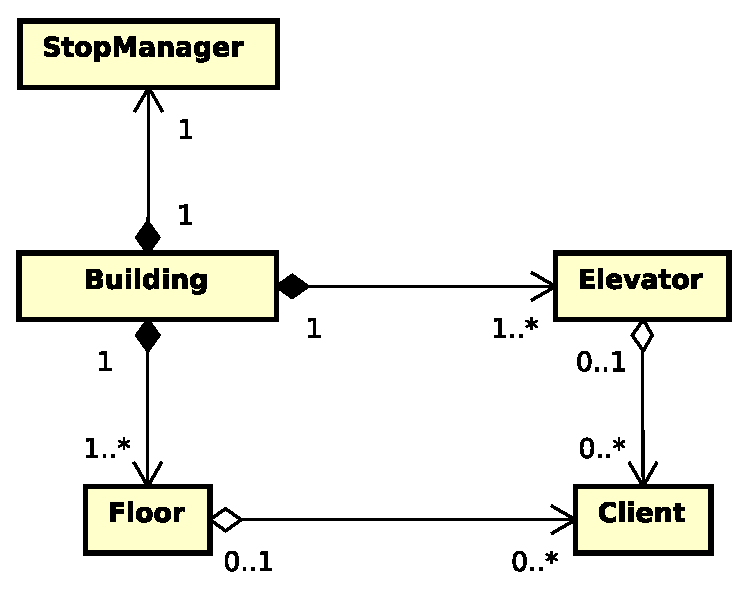
\includegraphics[scale=0.6]{img/Building}
  \caption{Diagrama de classes do \textit{prédio}.}
\label{fig:diagram:model}
\end{figure}

\section{\label{model:schedulers}Algoritmos de Agendamento}

Neste trabalho, dois algoritmos de agendamento foram implementados, o
\textit{Simple Scheduler} (Seção~\ref{model:schedulers:simple}) e o
\textit{Planning Scheduler} (Seção~\ref{model:schedulers:planning}). Ambos são
implementados em classes próprias, que herdam de uma classe \texttt{Scheduler}.
Este relacionamento pode ser visto mais claramente na
Figura~\ref{fig:model:schedulers:uml:base}.

\begin{figure}[htb!]
  \centering
  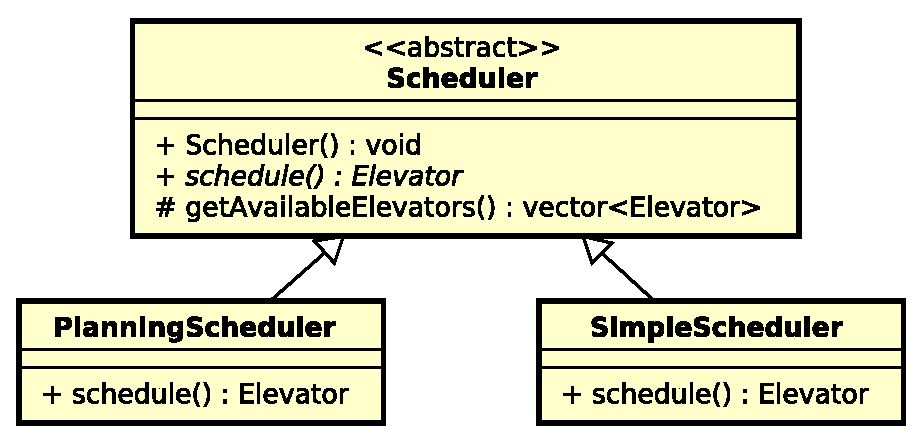
\includegraphics[scale=0.6]{img/Scheduler}
  \caption{Diagrama de classes das \textit{estratégias de agendamento}.}
  \label{fig:model:schedulers:uml:base}
\end{figure}

Os \textit{schedulers} têm apenas um método público, chamado \texttt{int
 schedule()}, que recebe como parâmetro a função de custo e um ponteiro para o
prédio, além de, opcionalmente, um elevador para ser excluído.

Excluir um elevador é importante, como foi falado na Seção
\ref{alg:building:state:update}. Há um método protegido na classe
\texttt{Scheduler}, chamado \texttt{getAvailableElevators()}, que retorna uma
lista de elevadores, excluindo aqueles que não podem ser utilizados.

\unsure{Talvez seja melhor explicar estes métodos seguindo o padrão utilizado nas seções anteriores para explicar as demais classes a manter o padrão.}

\subsection{\label{model:schedulers:simple}Simple}
O \textit{Simple Scheduler}, como o nome sugere, tem um comportamento bem
simples: itera pela lista de elevadores disponíveis, calculando a função de
custo para cada um, e retorna o de menor custo.

\unsure{Colocar algoritmo.}

\subsection{\label{model:schedulers:planning}Planning}
\lipsum[5]

\unsure{Colocar algoritmo.}

\section{\label{model:costfunctions}Algoritmos de Função de Custo}
As funções de custo herdam de uma classe base, chamada \texttt{CostFunction},
que possui apenas um método público, \texttt{float calculate()}, que retorna o
valor da função para aquela combinação entre o elevador e o cliente. Isto pode
ser visto em mais detalhes na Figura~\ref{fig:model:costfunction:uml:base}.

\unsure{Talvez seja melhor explicar estes métodos seguindo o padrão utilizado nas seções anteriores para explicar as demais classes a manter o padrão.}

\begin{figure}[htb!]
  \centering
  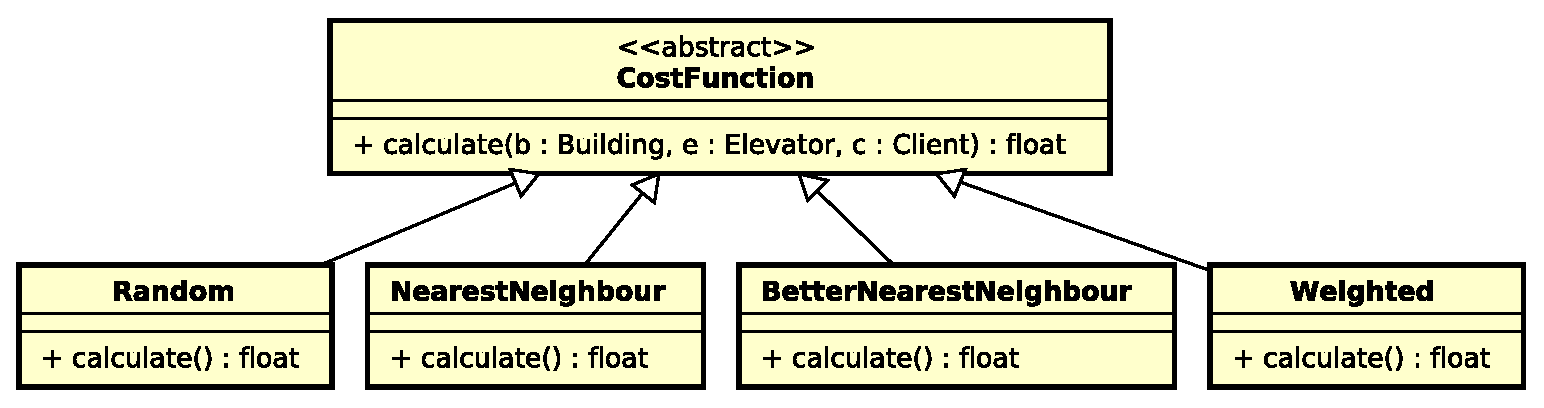
\includegraphics[scale=0.6]{img/CostFunction}
  \caption{Diagrama de classes das \textit{funções de custo}.}
  \label{fig:model:costfunction:uml:base}
\end{figure}

\subsection{\label{model:costfunctions:random}Random}

A Função de Custo \textit{Random} serve como base de comparação para as demais.
Ela retorna um valor aleatório entre zero e o número de andares do prédio cada
vez que for chamada, e, portanto, espera-se como resultado um agendamento não
ótimo.

Olhando-se a Figura~\ref{fig:model:costfunction:uml:base}, nota-se que ela é a
única função de custo com um construtor. Isto se dá por que é necessário
inicializar-se a geração de números aleatórios, de modo a gerar estes números de
forma consistente.

\begin{algorithm}[htb!]
  \centering
  \begin{minted}[linenos,fontsize=\small]{c++}

RandomCostFunction::RandomCostFunction()
 : _seed("54TH7hboAG1iOsDIDhJp")
 , _seed_seq(_seed.begin(), _seed.end())
 , _generator(_seed_seq)
{}

float RandomCostFunction::calculate(
    Building building,
    Elevator elevator,
    Client client) {

  if (_distribution == nullptr) {
    auto number_of_floors = building.getSimulator().getScenario().getFloorCount();
    _distribution = (0.0, number_of_floors);
  }

  auto dist = *_distribution;
  return dist(_generator);
}
  \end{minted}
  \caption{\label{alg:random_cf}Algoritmo de Função de Custo \textit{Random}.}
\end{algorithm}

\subsection{\label{model:costfunctions:nn}Nearest Neighbour}
Esta função de custo retorna, como custo, a distância do
elevador para o cliente. Ela ignora a direção na qual o elevador está viajando.

\begin{algorithm}[htb!]
  \centering
  \begin{minted}[linenos,fontsize=\small]{c++}
float NearestNeighbourCostFunction::calculate(
      Building building,
      Elevator elevator,
      Client client) {

    where_it_is = elevator.getLocation();
    where_to = client.getArrivalFloor();
    distance = where_it_is - where_to;

    return abs(distance);
}
  \end{minted}
  \caption{\label{alg:nn_cf}Função de custo \textit{nearest neighbour}.}
\end{algorithm}

\subsection{\label{model:costfunctions:bnn}Better Nearest Neighbour}
A Função de Custo \textit{Better Nearest Neighbour} bonifica elevadores que
estão indo na direção do chamado, dividindo seu custo por $\sqrt 2$ e bonifica
mais ainda os elevadores parados, dividindo seu custo por $2$. O custo antes
deste bônus é calculado de maneira igual à \textit{Nearest Neighbour}.

\begin{algorithm}[htb!]
  \centering
  \begin{minted}[linenos,fontsize=\small]{c++}
float BetterNearestNeighbourCostFunction::calculate(
      Building building,
      Elevator elevator,
      Client client) {

    auto where_it_is = elevator.getLocation();
    auto where_to = client.getArrivalFloor();
    auto distance = where_it_is - where_to;

    auto floors = building.getFloors();
    auto current_floor = floors.at(where_it_is);
    auto request_floor = floors.at(where_to);

    if (elevator.getStatus() == Status::Idle)
      return abs(distance) / sqrt(4.0);

    if (elevator.getDirection() == current_floor.compareTo(request_floor))
      return abs(distance) / sqrt(2.0);

    return abs(distance);
}
  \end{minted}
  \caption{\label{alg:bnn_cf}Função de Custo \textit{Better Nearest Neighbour}.}
\end{algorithm}

\subsection{\label{model:costfunctions:weighted}Weighted}
A Função \textit{Weighted} toma uma decisão diferente da \textit{Better Nearest
  Neighbour} para melhorar a \textit{Nearest Neighbour}. Em vez de bonificar
elevadores parados ou elevadores que estão indo na direção do cliente, esta
função bonifica elevadores mais vazios, dividindo o custo (que é a distância
entre o cliente e o elevador) pela ocupação do elevador.\footnote{Como foi visto
no Capítulo~\ref{chap:ai}, podemos inferir a ocupação pela balança interna do elevador, em
alguns cenários reais.}

\begin{algorithm}[htb!]
  \centering
  \begin{minted}[linenos,fontsize=\small]{c++}
float WeightedCostFunction::calculate(
      Building building,
      Elevator elevator,
      Client client) {

    if (elevator->getOccupation() == 0.0)
      return abs(client.getArrivalFloor() - elevator.getLocation());

    return abs(client.getArrivalFloor() - elevator.getLocation())
               / sqrt(elevator->getOccupation());
}
  \end{minted}
  \caption{\label{alg:weighted_cf}Função de Custo \textit{Weighted}.}
\end{algorithm}

\section{Geração de Relatórios} \label{model:report}

A cada fim de simulação, os \textit{contadores estatísticos} resultantes são
armazenados em uma coleção dentro da classe \texttt{Reporter}. Esta classe é
responsável por gerar relatórios da simulação. A listagem~\ref{alg:output}
mostra um exemplo de estrutura de diretórios e arquivos de saída.

\begin{listing}[H]
\dirtree{%
.1 output.
.2 High-rise\DTcomment{Nome do cenário.}.
.3 1 Simple Random\DTcomment{Diretório da estratégia.}.
.4 run.log\DTcomment{Log de execução da estratégia.}.
.4 report.log\DTcomment{Relatório das métricas da estratégia.}.
.4 trips.log\DTcomment{Arquivo contendo os desembarques de clientes.}.
.3 \ldots.
.3 arrivals.log\DTcomment{Arquivo contendo as chegadas de clientes.}.
.3 report.log\DTcomment{Relatório unificado de todas as estratégias do cenário.}.
}
\caption
   {\label{alg:output}Estrutura de diretórios e arquivos de saída.}
\end{listing}

\begin{description}[leftmargin=!,labelwidth=\widthof{\bfseries Arquivo de Desembarques}]
\item[Log de Execução]
O \textit{log de execução} apresenta o histórico da simulação,
mostrando sequencialmente o fluxo de processamento, ocorrência de eventos e
registro de decisões realizadas dentro do simulador.

\item[Métricas da Estratégia]
O \textit{relatório de métricas da estratégia} apresenta as métricas calculadas
para a simulação do cenário utilizando uma estratégia de agendamento específica.

\item[Arquivo de Desembarques]
O \textit{arquivo de desembarques} apresenta os dados de todos os desembarques
realizados para a simulação do cenário utilizando uma estratégia de agendamento
específica. Este arquivo é utilizado para a geração de gráficos.

\item[Arquivo de Chegadas]
O \textit{arquivo de chegadas} apresenta os dados de todas as chegadas de
clientes para a simulação do cenário utilizando uma estratégia de agendamento
específica. Este arquivo é utilizado para a geração de gráficos.

\item[Relatório Unificado]
O \textit{relatório unificado} apresenta as métricas geradas por todas as
estratégias selecionadas para simulação de um cenário. Assim, fornece um meio de
observar e analisar os resultados obtidos.

\end{description}

\subsection{\label{model:report:charts}Geração de Gráficos}

Os gráficos são gerados a partir do arquivo de desembarques. A
Listagem~\ref{alg:graphs:output} mostra um exemplo de estrutura de diretórios e
arquivos de saída.

\begin{listing}[H]
\dirtree{%
.1 output.
.2 High-rise\DTcomment{Nome do cenário.}.
.3 1 Simple Random\DTcomment{Diretório da estratégia.}.
.4 arrivalsPerFloor.eps\DTcomment{Chegadas por andar.}.
.4 averageTravelTime.eps\DTcomment{Tempo médio de jornada de andar para andar.}.
.4 averageWaitTime.eps\DTcomment{Tempo médio de espera por andar.}.
.4 clientsPerElevator.eps\DTcomment{Total de clientes em cada elevador.}.
.4 dropoffsPerFloor.eps\DTcomment{Total de clientes entregues em cada andar.}.
}
\caption
   {\label{alg:graphs:output}Estrutura de diretórios e arquivos de saída.}
\end{listing}

Um script em Python é chamado para cada arquivo de desembarques, de modo a
processá-lo e gerar estes gráficos.

